\section{Application} \label{sec:application}
In order to test the self-developed deviation evaluation method from the previous \cref{sec:implementation}, the following section presents the experimental setup used to acquire dynamic phases of time-resolved electron waves for a specific set of gate length $\tau$ and sampling resolution $t_0$, derive their slopes and compare them to the time-discrete data points for the three previously detailed signals.
\subsection{Experiment} \label{ssec:application-experiment}
All measurements\footnote{Due to the COVID-19 pandemic, all measurements and pictures were graciously provided by the supervisor.} were done with the FEI Titan™ 80-300 Berlin Holography Special TEM (\cref{fig:FEI-Titan}) in a special extended Lorentz holography mode \cite{Wagner2019}. All holograms for the coplanar capacitor (\cref{fig:EH-biased}), which was cut from a micro-electro-mechanical system (MEMS) chip with a FEI Helios NanoLab™ 600 and placed in a DENSsolution Wildfire™ S3 In Situ TEM Heating System (\cref{fig:TEM-Holder}), were captured with a Gatan UltraScan™ 1000 CCD Camera for an exposure time $T_{exp}$ and an acceleration voltage $U_a$. The capacitor was externally biased with $U_{ext}$ and measurements with $U_{ext} = \SI{0}{\volt}$ were used as empty holograms. A GW Instek™ GDS-1102B Digital Oscilloscope was used to monitor the applied signal.
\begin{figure}[H]
	\centering
	\begin{subfigure}[c]{\textwidth}
		\centering
		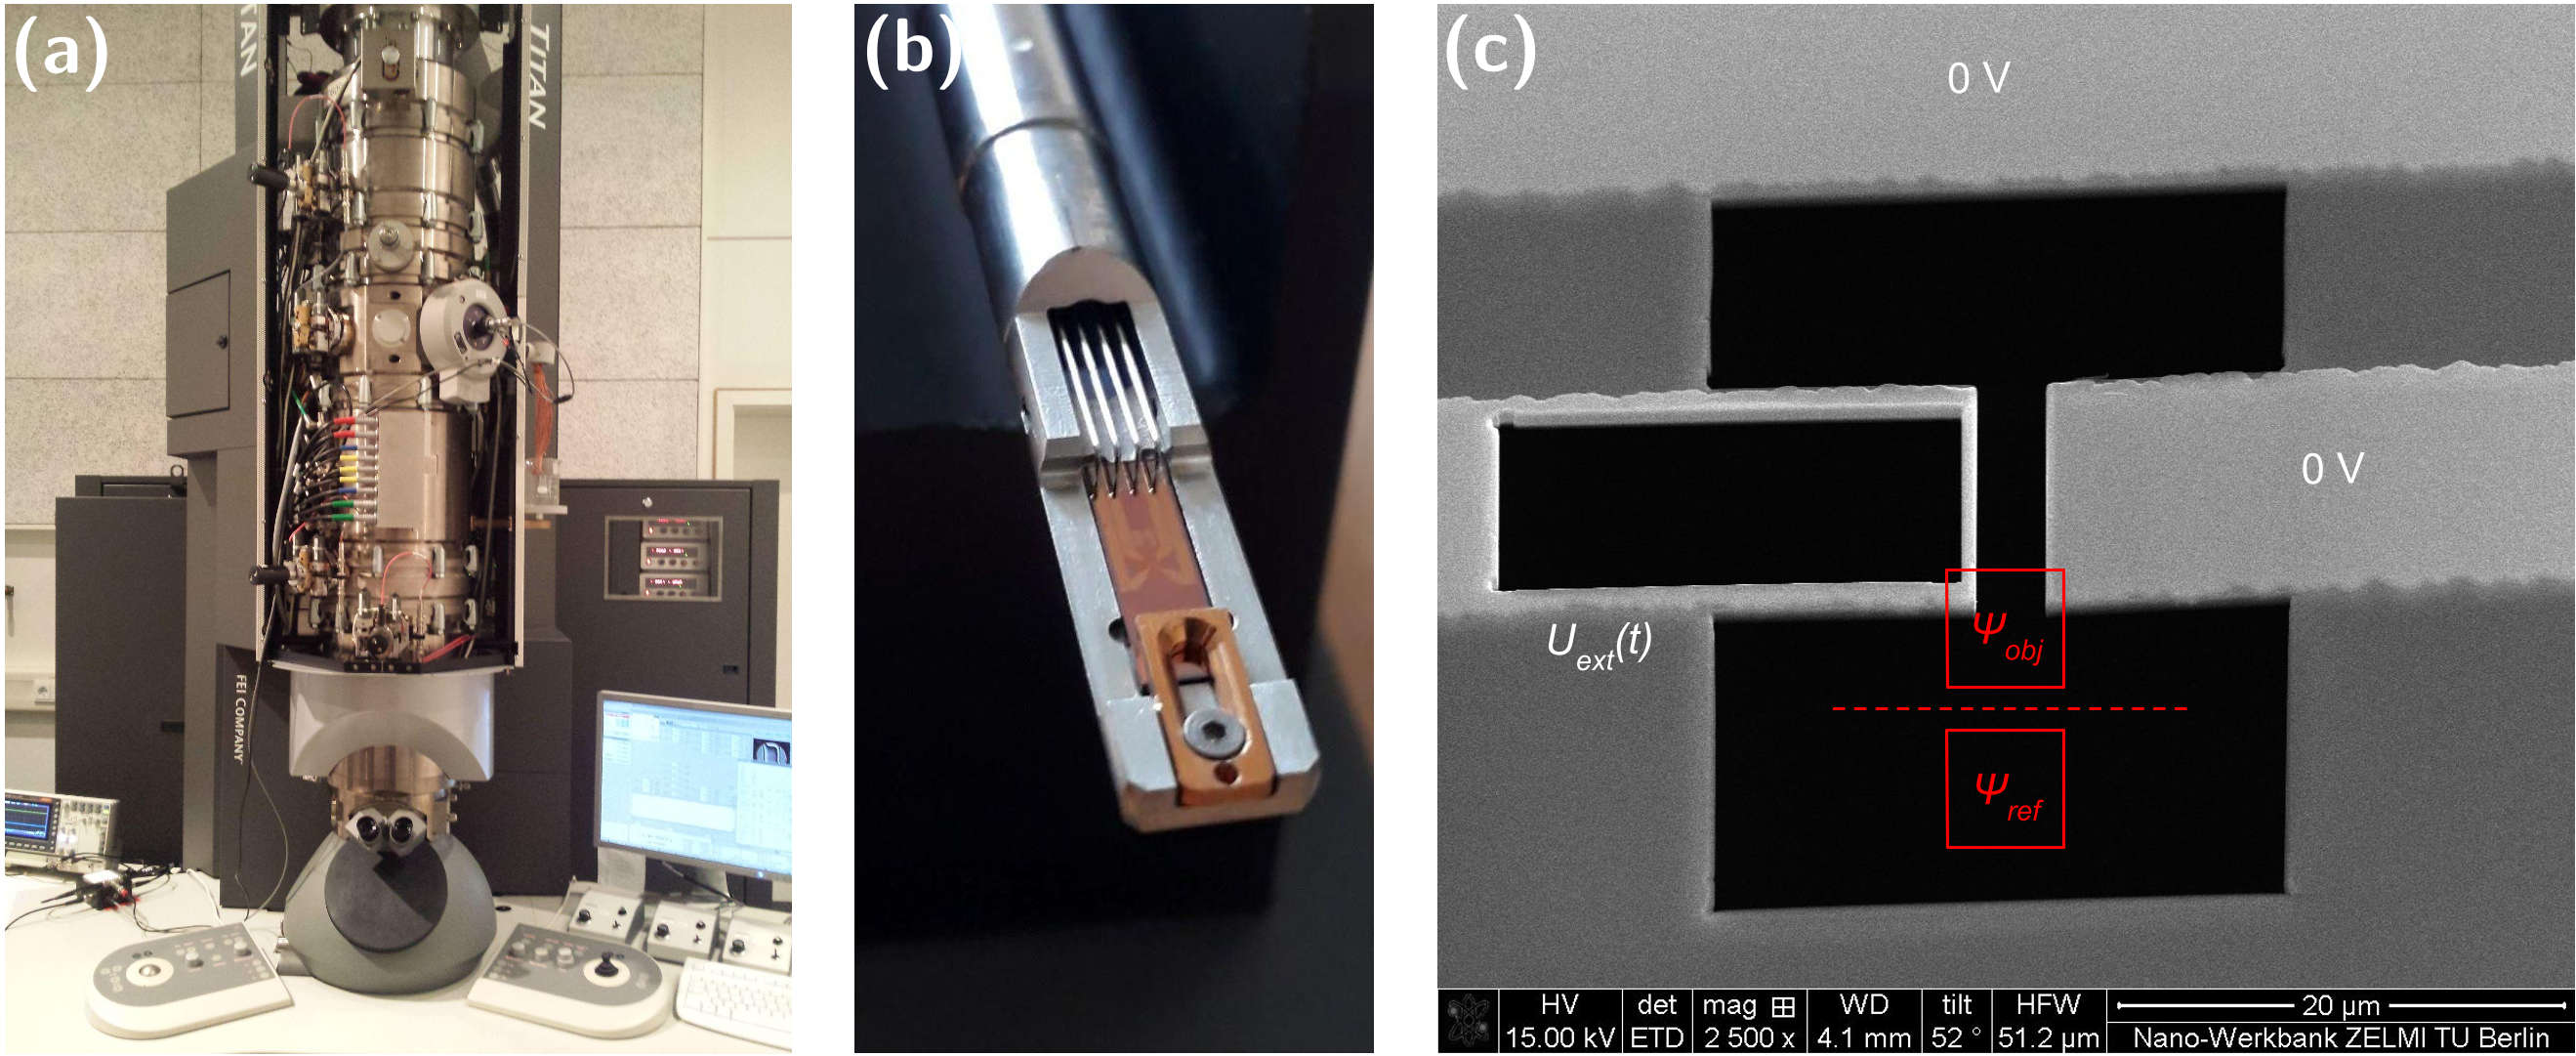
\includegraphics[width=\textwidth]{Figures/Setup.pdf}
		\phantomsubcaption
		\label{fig:FEI-Titan}
	\end{subfigure}%
	\begin{subfigure}[c]{0\textwidth}
		\centering
		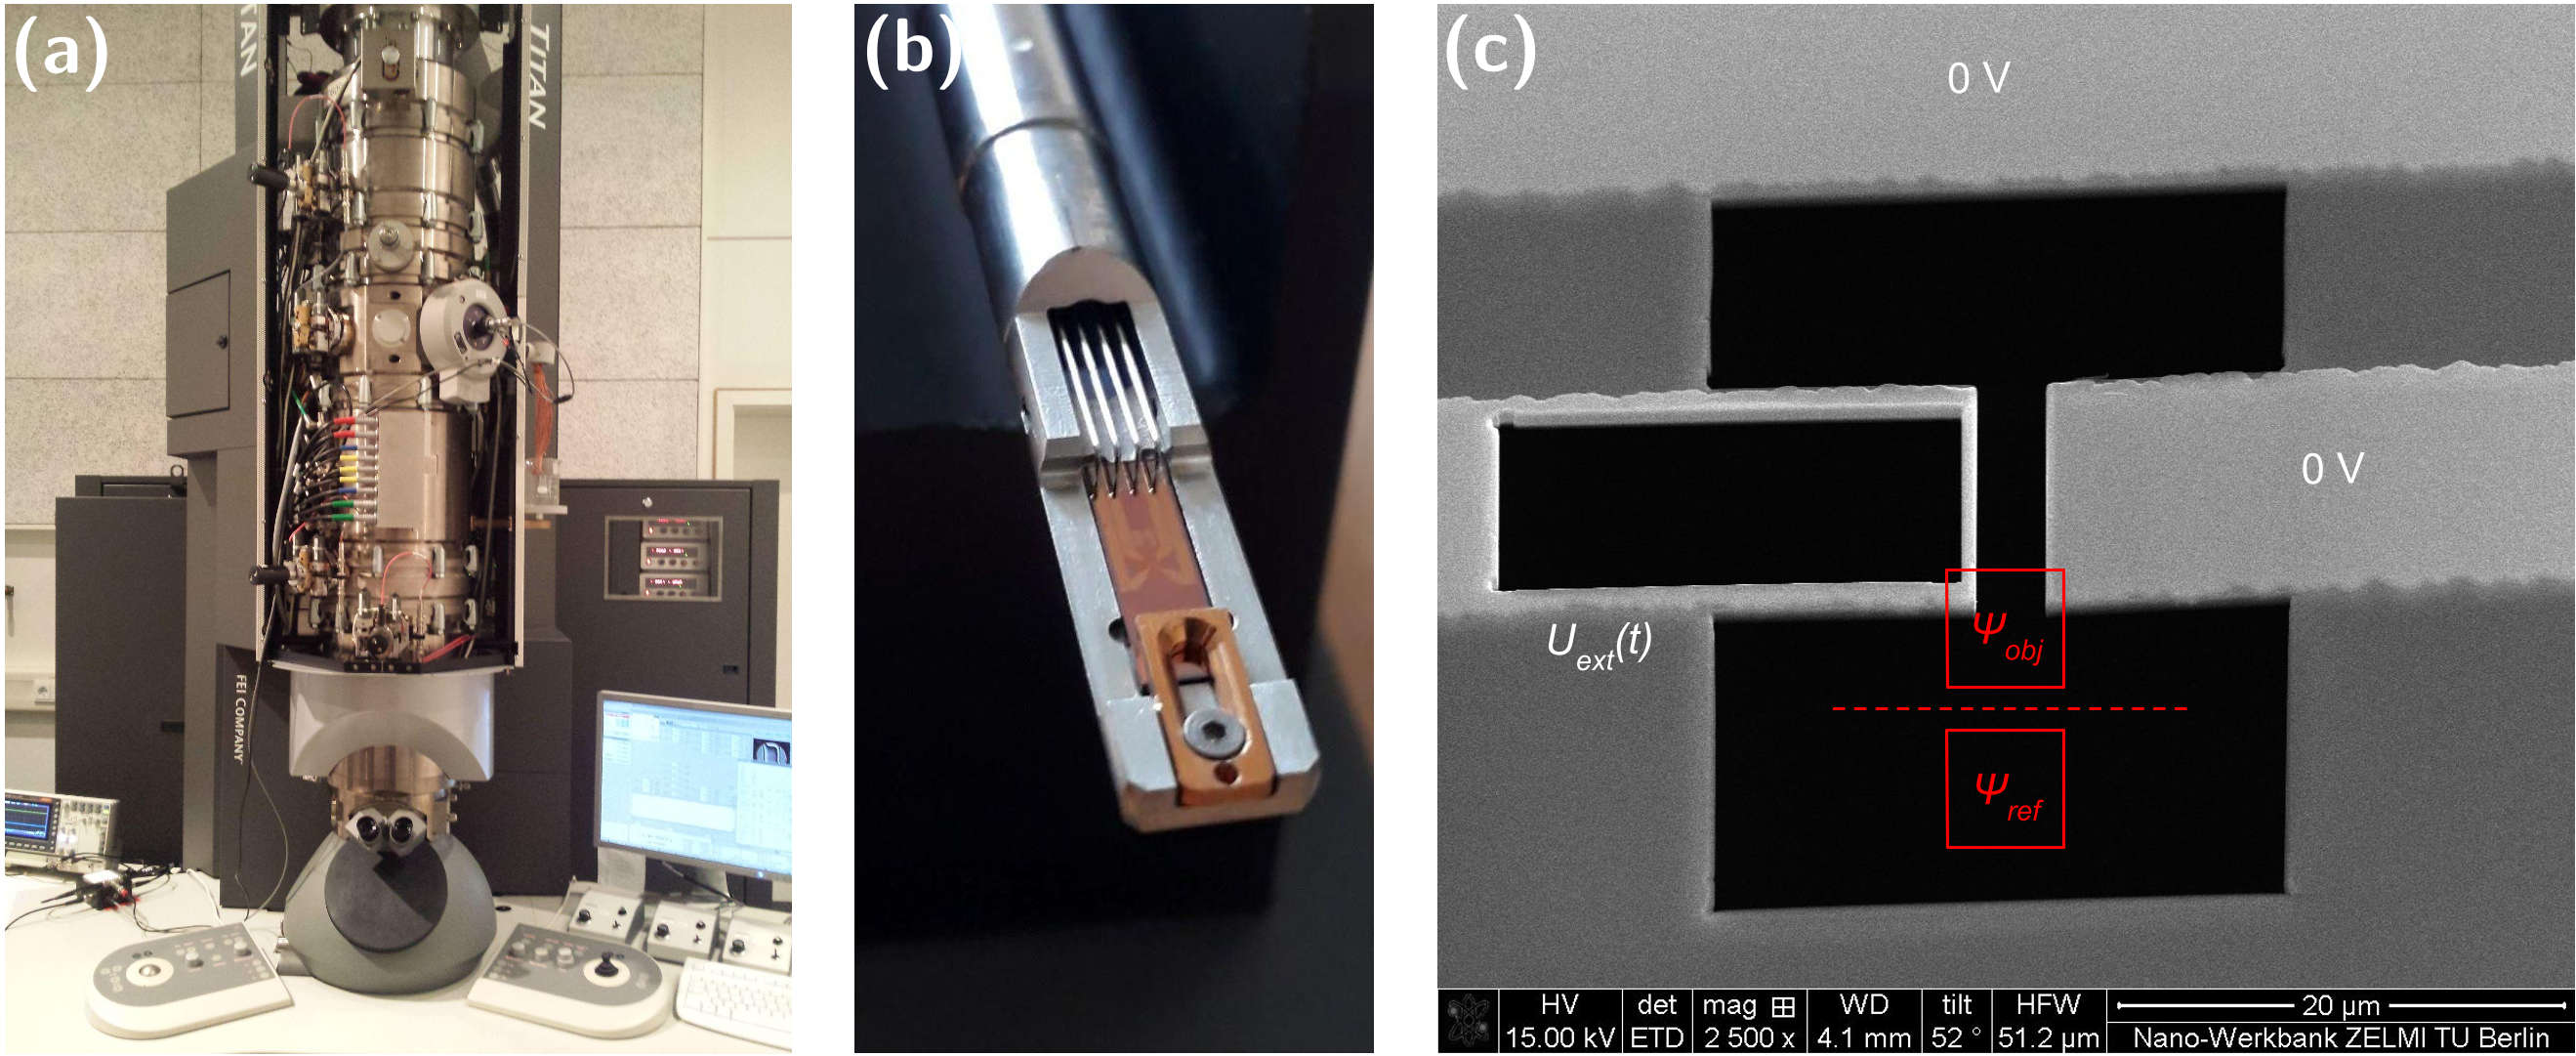
\includegraphics[width=\textwidth]{Figures/Setup.pdf}
		\phantomsubcaption
		\label{fig:TEM-Holder}
	\end{subfigure}%
	\begin{subfigure}[c]{0\textwidth}
		\centering
		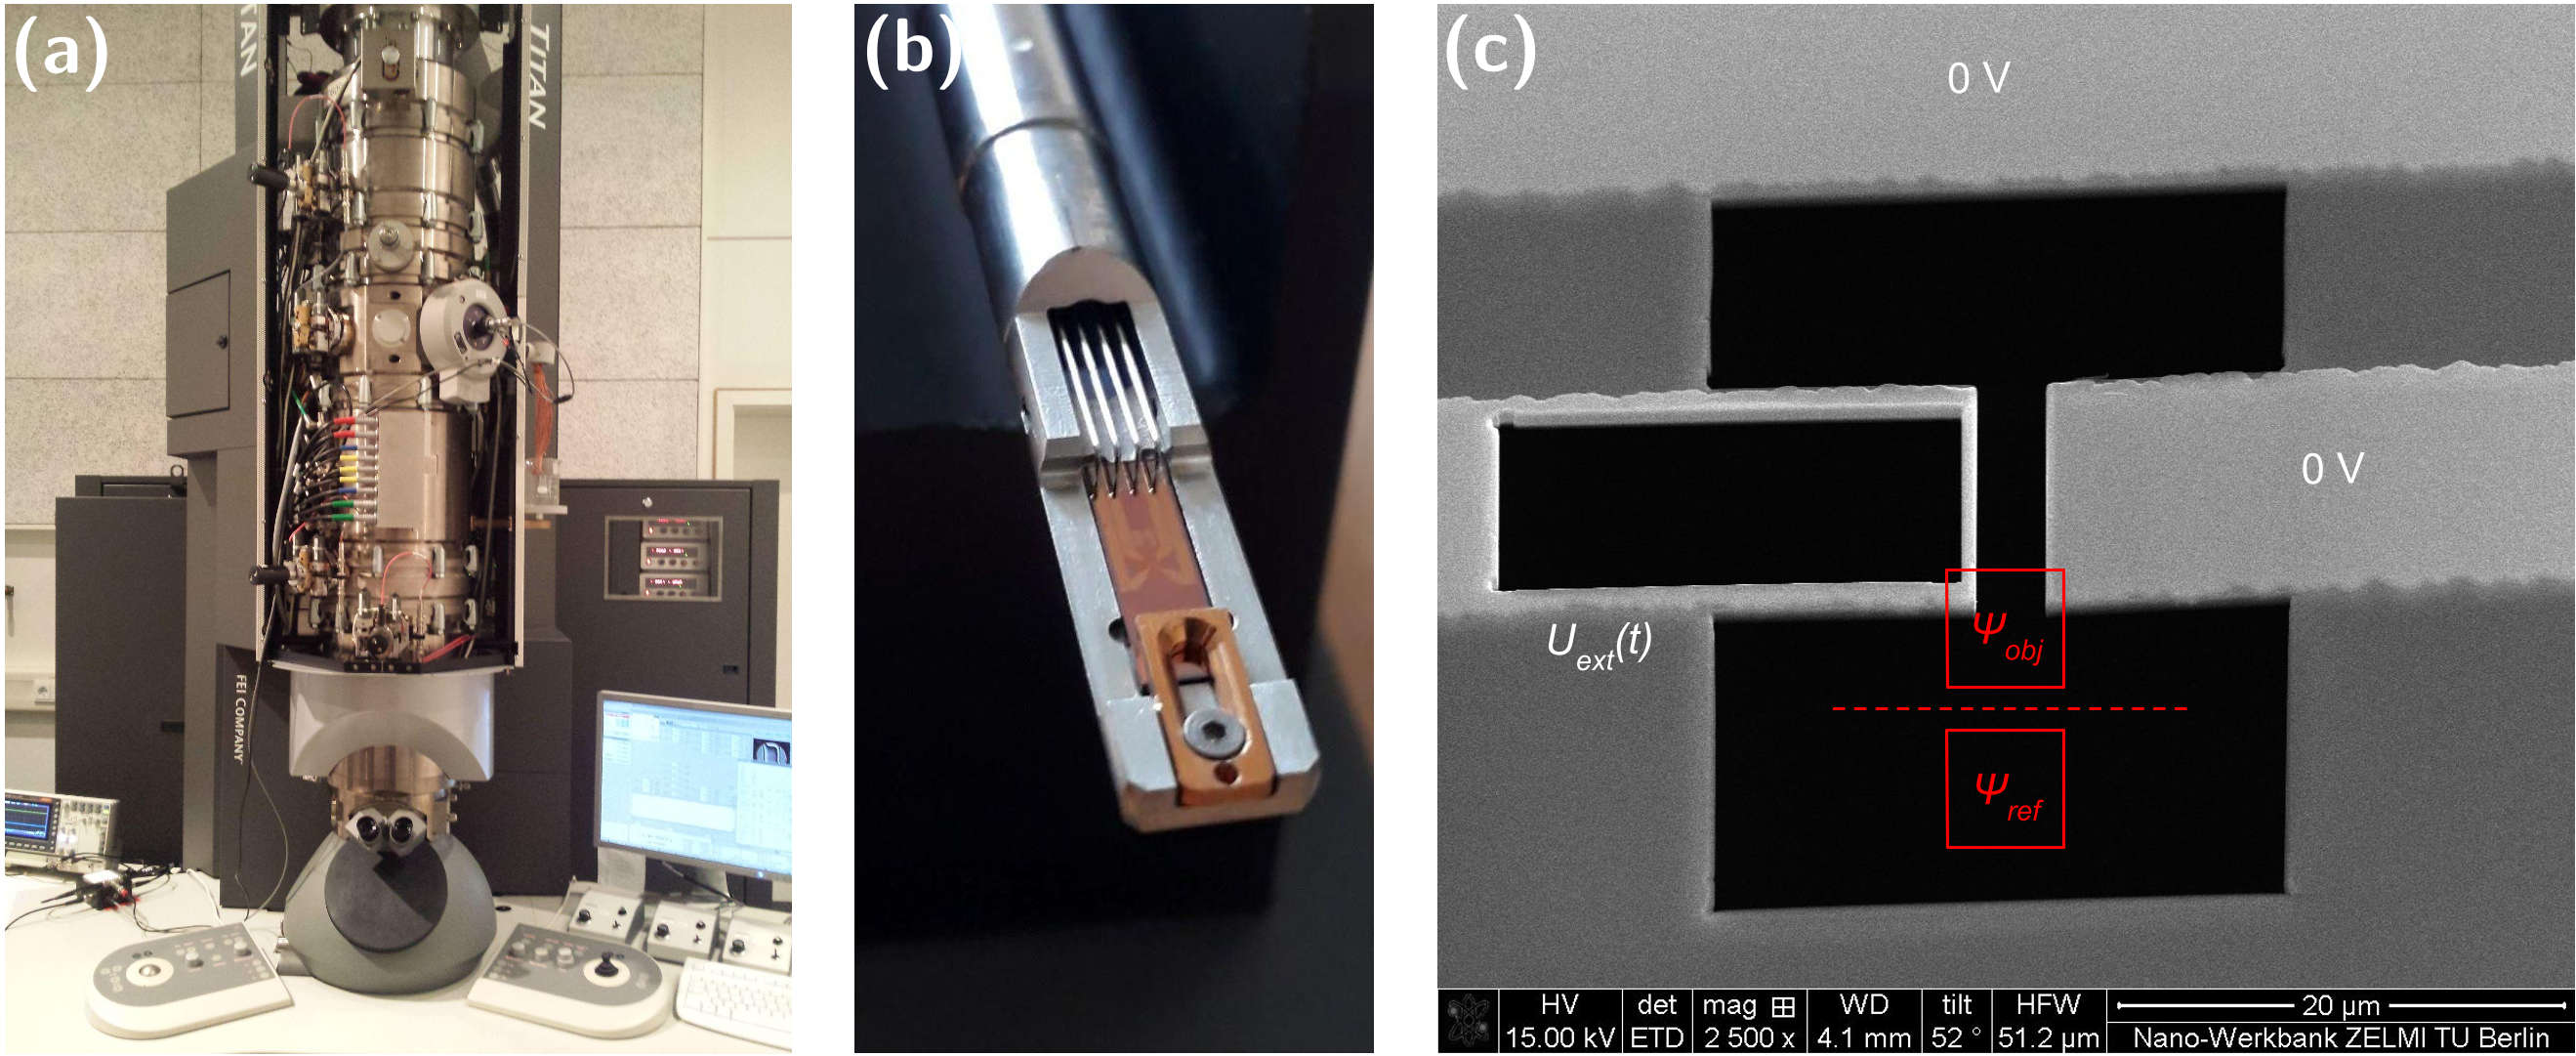
\includegraphics[width=\textwidth]{Figures/Setup.pdf}
		\phantomsubcaption
		\label{fig:Capacitor-SEM}
	\end{subfigure}%
	\caption{Experimental setup featuring the (a) FEI Titan™ 80-300 Berlin Holography Special TEM, (b) DENSsolution Wildfire™ S3 In Situ TEM Heating System and (c) SEM micrograph of the coplanar capacitor with the position of the biprism (dashed line) marked for the respective electron holography setup.}
	\label{fig:Experiment-Setup}
\end{figure}
By using focused ion beam milling, the required capacitor can be manufactured from a MEMS chip by cutting through a conductive trace and milling a window into the adjacent silicon nitride diaphragm. Both ends of the severed trace, which is made of a $\SI{200}{\nano\metre}$ thick Au layer covered in $\SI{200}{\nano\metre}$ thick Si\textsubscript{3}Ni\textsubscript{4} layers, make up the terminals of the capacitor (\cref{fig:Capacitor-SEM}) with a distance of $\SI{2.75}{\micro\metre}$ in between and a width of $\SI{15}{\micro\metre}$.

Then, the capacitor is placed in an in situ TEM holder, which provides a mechanical and electrical connection using spring contacts and a cooper latch (\cref{fig:TEM-Holder}).

Biasing the left terminal with the external voltage $U_{ext}$ while grounding the right terminal leads to a capacitor with a one sided potential that varies between $+U_{ext}$ and $-U_{ext}$ for an AC voltage source (\cref{fig:Capacitor-SEM}). The electric potential of the capacitor leads to a modulation of the phase $\varphi\left(\vb{r}\right)$ regarding the image wave ${\psi}_{rec}\left(\vb{r}\right)$ \cite{Niermann2017}.

In order to improve the signal-to-noise ratio, multiple holograms with $U_{ext} = \text{const}$ are captured and then averaged for every gate position $t_{g_j}$. The phase slope $\dv*{}{x} \varphi\left(x\right)$, which is proportional to the external voltage $U_{ext}$, is calculated by defining a rectangular area in between both terminals of the capacitor, determining the gradient through the distance of adjacent pixels and projecting it onto the connecting vector going from the grounded terminal to the biased one. The error of the phase slope follows by calculating the variance.
\subsection{Results} \label{ssec:application-results}
With the phase slope being proportional to the capacitor voltage (i.\,e. $\dv*{}{x} {\varphi}_{t_{g_j}}\left(x\right) \sim U_{ext}\left(t_{g_j}\right)$), the question of direct comparison to the oscilloscope signal $U\left(t\right)$ arises.

Starting with the sine wave signal, where the measurement uses an acceleration voltage of $U_a = \SI{300}{\kilo\volt}$, an exposure time of $T_{exp} = \SI{3}{\second}$ each and averages five consecutive holograms, as well as a gate length of $\tau = 0.1T$ and sampling resolution of $t_0 = 0.05T$ for both the phase slopes and the time-discrete data points, both $\dv*{}{x} {\varphi}_{t_{g_j}}\left(x\right)$ and $\overline{U}_j\left(t_{g_j}\right)$ constitute an accurate representation of the oscilloscope signal (\cref{fig:sine-slope}). Not only do all values for the phase slope have little to no deviation from the time-discrete points, but the attenuating effect of the temporal discretization on the amplitude is also non-present for the specified parameters.
\begin{figure}[H]
	\centering
	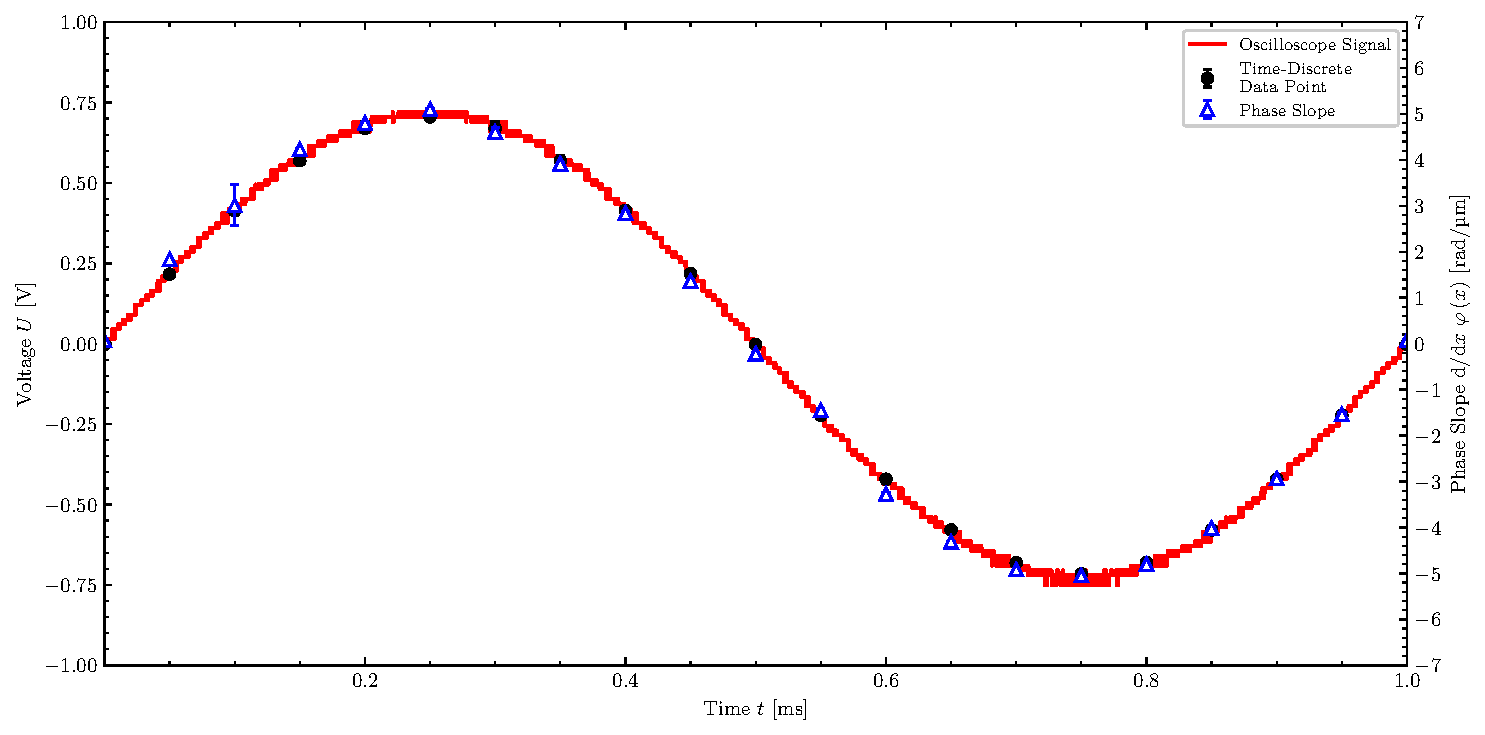
\includegraphics[width=0.75\textwidth]{Figures/Slope/sine_slope.pdf}
	\caption{Plot of the oscilloscope sine wave signal $U\left(t\right)$ along with the phase slopes $\dv*{}{x} \varphi\left(x\right)$ at $t_{g_j}$ and the time-discrete data points $\overline{U}_j\left(t_{g_j}\right)$ for a gate length of $\tau = 0.1T$ and a sampling resolution of $t_0 = 0.05T$.}
	\label{fig:sine-slope}
\end{figure}
The same measurement of the phase slopes $\dv*{}{x} \varphi\left(x\right)$, with a gate length $\tau = 0.1T$ and a sampling resolution of $t_0 = 0.05T$, can be done for the square wave signal (\cref{fig:square-slope}). Here, the acceleration voltage is set to $U_a = \SI{200}{\kilo\volt}$ with an exposure time of $T_{exp} = \SI{4}{\second}$ each for four consecutive holograms that are averaged.

Similar to the sine wave signal from above, both the phase slopes and the time-discrete data points provide an accurate representation of the oscilloscope square wave signal. The only noticeable deviations between the phase slopes and the time-discrete data points occur during the rise/fall time of the oscilloscope signal, where the phase slope is either almost identical to the oscilloscope signal and the time-discrete data point deviates, or both the phase slope and the time-discrete data point feature a similar deviation from the oscilloscope signal. It can be observed, however, that the measured phase slopes feature a phase wedge, which in turn causes $\abs*{\dv*{}{x} {\varphi}_{t_{g_j}}\left(x\right)}$ to be non-symmetric around zero. Furthermore, the oscilloscope signal features a plateau during the rise/fall time with a width of $\approx \SI{0.15}{\micro\second}$.

The discharge of the capacitor can be modeled using the exponential function \cite{carr2001}: $$U\left(t\right) = U_{pp} \cdot e^{-\frac{t}{R\cdot C}}$$ and the measured capacitance $C$ and resistance $R$. Connecting an ohmmeter directly to the MEMS chip prior to cutting through the conductive trace allows for a measurement of the resistance with $R = \SI{392 \pm 20}{\ohm}$, while a Keysight™ E4980A Precision LCR Meter can be used to measure the capacitance at $C = \SI{152 \pm 20}{\pico\farad}$ in a frequency range of $\SIrange{70}{700}{\kilo\hertz}$ \cite{Wagner2018}.
\begin{figure}[H]
	\centering
	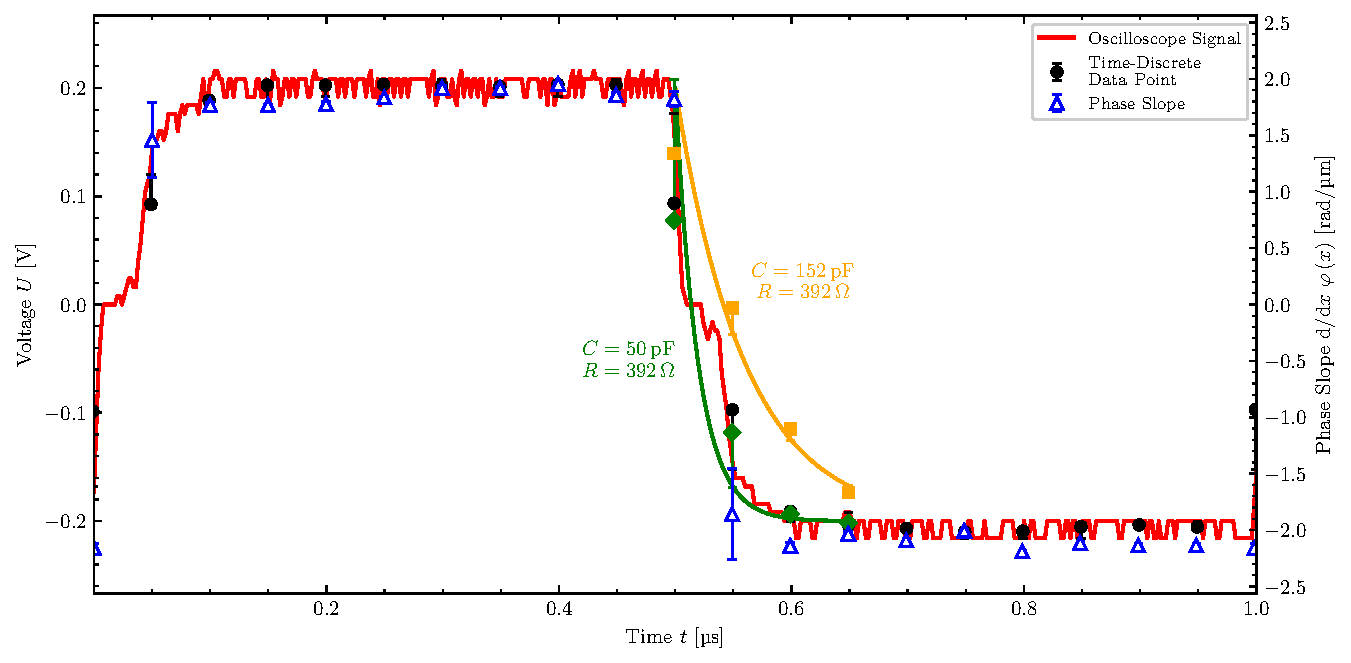
\includegraphics[width=0.75\textwidth]{Figures/Slope/square_slope.pdf}
	\caption{Plot of the oscilloscope square wave signal $U\left(t\right)$ along with the phase slopes $\dv*{}{x} \varphi\left(x\right)$ at $t_{g_j}$ and the time-discrete data points $\overline{U}_j\left(t_{g_j}\right)$ for a gate length of $\tau = 0.1T$ and a sampling resolution of $t_0 = 0.05T$. Moreover, an exponential function can be used for the discharge of the capacitor between $\SI{0.5}{\micro\second}$ and $\SI{0.65}{\micro\second}$ to demonstrate the fall time for different capacitances $C$ and constant resistance $R$.}
	\label{fig:square-slope}
\end{figure}
With these parameters, it is apparent that the modeled curve is falling too slow to approximate the capacitor, causing the time-discrete data points from $\SIrange{0.55}{0.65}{\micro\second}$ to distance themselves from the phase slopes. Assuming the capacitance at $C =\SI{50}{\pico\farad}$ causes the resulting time-discrete data points to move closer to the phase slopes.

At last, the same measurement of the phase slopes $\dv*{}{x} \varphi\left(x\right)$, with a gate length $\tau = 0.1T$ and a sampling resolution of $t_0 = 0.05T$, can be done for the Bat-Signal (\cref{fig:batman-slope}). Here, the acceleration voltage is set to $U_a = \SI{300}{\kilo\volt}$ with an exposure time of $T_{exp} = \SI{3}{\second}$ each for five consecutive holograms that are averaged, identical to the square wave signal.
\begin{figure}[H]
	\centering
	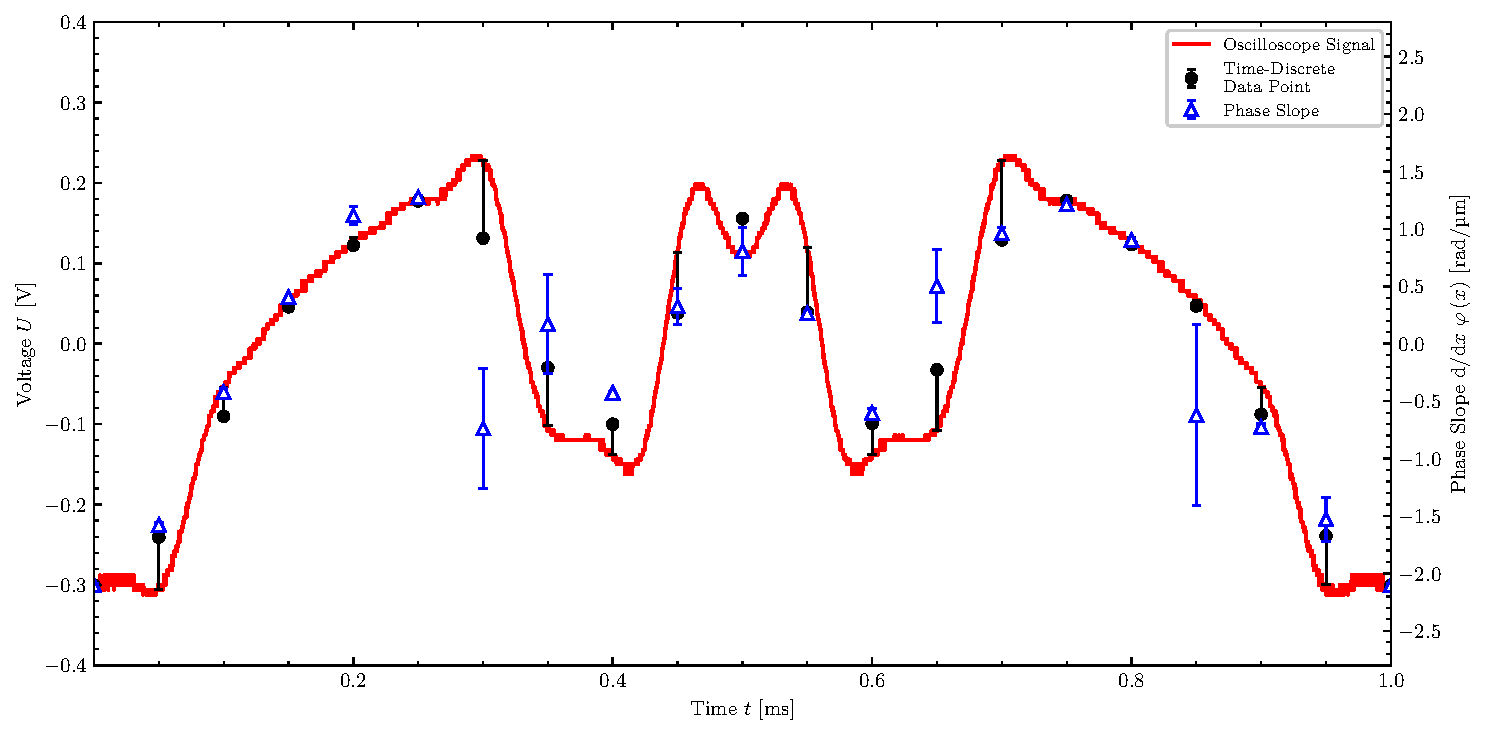
\includegraphics[width=0.75\textwidth]{Figures/Slope/batman_slope.pdf}
	\caption{Plot of the oscilloscope Bat-Signal $U\left(t\right)$ along with the phase slopes $\dv*{}{x} \varphi\left(x\right)$ at $t_{g_j}$ and the time-discrete data points $\overline{U}_j\left(t_{g_j}\right)$ for a gate length of $\tau = 0.1T$ and a sampling resolution of $t_0 = 0.05T$.}
	\label{fig:batman-slope}
\end{figure}
The complicated Bat-Signal, with its rapid changes in amplitude and slope along with the symmetry of the signal, features a wider array of deviations between the phase slopes, the time-discrete data points and the oscilloscope signal. The areas of steady rise or decline (i.\,e. $\SIrange{0}{\approx 0.3}{\milli\second}$ and $\SIrange{\approx 0.7}{1.0}{\milli\second}$) feature only small deviations between the phase slopes and the time-discrete data points, with both of them bordering on the oscilloscope signal. The phase slopes for $t_{g_j} = \SI{0.3}{\milli\second}$ and $t_{g_j} = \SI{0.85}{\milli\second}$ show major deviations from the time-discrete data points, which are neighboring the oscilloscope signal. Furthermore, the sections of sharp rise or decline (i.\,e. $\SIrange{\approx 0.3}{\approx 0.4}{\milli\second}$ and $\SIrange{\approx 0.6}{\approx 0.7}{\milli\second}$) show less deviation between the phase slopes and time-discrete data points than between the phase slopes and the oscilloscope signal, adhering to the above established presumption of the phase slopes being closer to the time-discrete data points. The middle section of the signal featuring the spikes (i.\,e. $\SIrange{\approx 0.4}{\approx 0.6}{\milli\second}$) shows the same behavior, with the exception of the phase slope located at exactly the middle of the signal (i.\,e. $t_{g_j} = \SI{0.5}{\milli\second}$), for which the phase slope is closer to the oscilloscope signal than to the time-discrete data point.
\subsection{Discussion} \label{ssec:application-discussion}
The sine wave signal, being the simplest case to measure, shows little to no deviation of both the phase slopes and the time-discrete data points from the oscilloscope signal for a gate length of $\tau = 0.1T$ and a sampling resolution of $t_0 = 0.05T$. Therefore, the comparison between the phase slopes and the oscilloscope signal can be made without further considerations, as predicted by the self-developed method.

The square wave signal, however, features deviations during the rise/fall time of the oscilloscope signal where the capacitor is (dis-)charging. Here, the plateau with a width of $\approx \SI{0.15}{\micro\second}$ is caused by both capacitive reflections on the conductive tracks and cables \cite{carr2001} and parasitic capacitances on the MEMS chip \cite{Wagner2018}.

The large error of the measured resistance $R$ and capacitance $C$ can likewise be attributed to the above mentioned parasitic capacitances and is depended on the thickness of the silicon nitride layer \cite{Wagner2018}. Nevertheless, the higher agreement of the exponential model for a capacitance of $C = \SI{50}{\pico\farad}$ with the oscilloscope signal, therefore causing the resulting time-discrete data points to move closer to the measured phase slopes, shows that the measured capacitance of $C = \SI{152 \pm 20}{\pico\farad}$ is more applicable to the whole MEMS chip rather than the single capacitor investigated. The deviation between the time-discrete data point and the phase slope at $t_{g_j} = \SI{0.5}{\micro\second}$ is due to \emph{overshooting}, an effect that only applies to the single capacitor, therefore only effecting the phase slope, instead of the whole MEMS chip \cite{Stewart2006}. This also shows that the interference gating method is an excellent candidate for measurements of single electronic components inside sophisticated circuits.

The deviations between the phase slopes, the time-discrete data points and the oscilloscope Bat-Signal are highly dependent on the measured section of the signal. The non-symmetric deviations of the phase slope for $t_{g_j} = \SI{0.3}{\milli\second}$ and $t_{g_j} = \SI{0.85}{\milli\second}$ can be attributed to a measurement error in the empty hologram caused by external fields. The deviation of the phase slope between the spikes of the signal is caused by high-frequency components, showing that a gate length of $\tau = 0.1T$ is pushing the limits of accurate representation. Furthermore, changes that are smaller than $0.5\tau$, such as narrow spikes in the signal, contribute to a large deviation of both the phase slopes and the time-discrete data points from the oscilloscope signal. Overall, both the phase slopes and the time-discrete data points still amount to a fairly accurate representation of the oscilloscope signal when selecting a gate length of $\tau = 0.1T$ and a sampling resolution of $t_0 = 0.05T$.

Following the above made observations, the temporal discretization based deviations of the interference gating method can be regarded as a lower bound error that is, regardless of experimental setup, always present. Therefore, the phase slopes are not only proportional, but also closer to the time-discrete data points (i.\,e. $\dv*{}{x} {\varphi}_{t_{g_j}}\left(x\right) \sim \overline{U}_j\left(t_{g_j}\right)$) than to the oscilloscope signal. Since perfect measurements are not feasible to achieve, various deviations that arise from different measurement errors have to be accounted for in addition to this lower bound error.